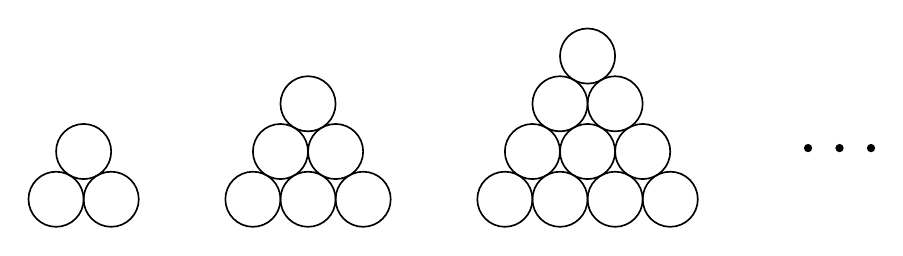
\begin{tikzpicture}[x=1cm,y=1cm,line width=.6pt,font=\normalsize]
% pile 1: 3 circles (rows 2+1), X=0.35
\draw (0.35,0.35) circle[radius=0.35cm];
\draw (1.05,0.35) circle[radius=0.35cm];
\draw (0.70,0.9562) circle[radius=0.35cm];
% pile 2: 6 circles (rows 3+2+1), X=2.85
\draw (2.85,0.35) circle[radius=0.35cm];
\draw (3.55,0.35) circle[radius=0.35cm];
\draw (4.25,0.35) circle[radius=0.35cm];
\draw (3.20,0.9562) circle[radius=0.35cm];
\draw (3.90,0.9562) circle[radius=0.35cm];
\draw (3.55,1.5624) circle[radius=0.35cm];
% pile 3: 10 circles (rows 4+3+2+1), X=6.05
\draw (6.05,0.35) circle[radius=0.35cm];
\draw (6.75,0.35) circle[radius=0.35cm];
\draw (7.45,0.35) circle[radius=0.35cm];
\draw (8.15,0.35) circle[radius=0.35cm];
\draw (6.40,0.9562) circle[radius=0.35cm];
\draw (7.10,0.9562) circle[radius=0.35cm];
\draw (7.80,0.9562) circle[radius=0.35cm];
\draw (6.75,1.5624) circle[radius=0.35cm];
\draw (7.45,1.5624) circle[radius=0.35cm];
\draw (7.10,2.1686) circle[radius=0.35cm];
% ellipsis
\fill (9.90,1.0) circle (1.5pt);
\fill (10.30,1.0) circle (1.5pt);
\fill (10.70,1.0) circle (1.5pt);
\end{tikzpicture}
